\begin{frame}
    \frametitle{3D Printing a Nuclear Reactor?}
    \begin{block}{Impact of Additive Manufacturing Technology Advancements on 
        Reactor Design Optimization}
        \begin{itemize}
            \item With further advancement of additive manufacturing technologies, a reactor 
            core could be 3D printed in the near future
            \item Leveraging additive manufacturing enables us to surpass classical 
            manufacturing constraints and optimize for arbitrary geometries and parameters 
            such as non-uniform channel shapes, and inhomogeneous fuel distribution 
            throughout the core
          \end{itemize}
    \end{block}
  \end{frame}

  \begin{frame}
    \frametitle{Evolutionary Algorithm Optimization}
    \begin{block}{Evolutionary Algorithms for Reactor Design Optimization}
    \begin{minipage}[c]{0.6\textwidth}
        \begin{itemize}
            \item We can leverage evolutionary algorithm optimization to 
            explore the large design space enabled by 3D printing to find global 
            optimal designs
            \item Evolutionary algorithms have proven successful in optimizing 
            multi-objective problems as they can find solutions at the global 
            optimum and can be run in parallel
            \item Evolutionary algorithms imitate natural selection to evolve solutions 
            \end{itemize}
  \end{minipage}\hfill
  \begin{minipage}[c]{0.4\textwidth}
    \centering
    \begin{figure}
      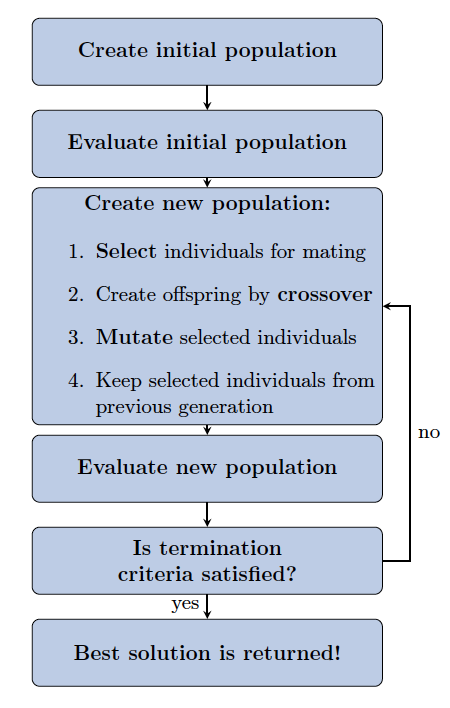
\includegraphics[width=0.8\linewidth]{figures/ea-flow.png} 
      \caption{Evolutionary algorithm flow \cite{renner_genetic_2003}. }
    \end{figure}
  \end{minipage}
  \end{block}
  \end{frame}
    